%-----------------------
% PREAMBLE
%-----------------------
\documentclass[compress]{beamer}

\useoutertheme{infolines}
\setbeamertemplate{headline}[default]
\setbeamertemplate{footline}{}
\mode<beamer>{\setbeamertemplate{blocks}[rounded][shadow=true]}
\setbeamercovered{transparent}
\setbeamercolor{block body example}{fg=blue, bg=black!20}
\useoutertheme[subsection=false]{miniframes}

\title{Augmented Reality (AR) Navigation System\\ for Commercial Spaces}
\author{Software Projects - Group 14}
\institute{Arif Kharoti, Nicholas Orford-Williams, Hardik Ramesh, \\Gabriel Sampaio Da Silva Diogo, Hamza Sheikh, Jonathan Tang}
\date{March 2019}

%-----------------------
% SLIDES
%-----------------------
\begin{document}
	\begin{frame}
		\titlepage
	\end{frame}

	\section{Motivation \& Scope}
	\subsection{Motivation}
	\begin{frame}
		\frametitle{Motivation}
		\begin{itemize}
			\item Lack of maps and signage in museums.
			\item Old technology currently in use, e.g. portable audio guides
			\item Various applications to other scenarios, e.g. supermarkets or libraries.
		\end{itemize}
	\end{frame}

	\subsection{Scope}
	\begin{frame}
		\frametitle{Scope}
	    \begin{itemize}
			\item Display navigational routes in real-time.
			\item Calculate the shortest route to the user specified location.
			\item Use AR to enhance user navigation routing.
		\end{itemize}
	\end{frame}

	\section{Design}
	\subsection{Design}
	\begin{frame}
		\frametitle{Design}
		\begin{itemize}
			\item Android Prototyping
			\item User flow diagrams
			\item Model-View Controller
		\end{itemize}
	\end{frame}

	\begin{frame}
		\framesubtitle{User Flow Diagrams}
		% 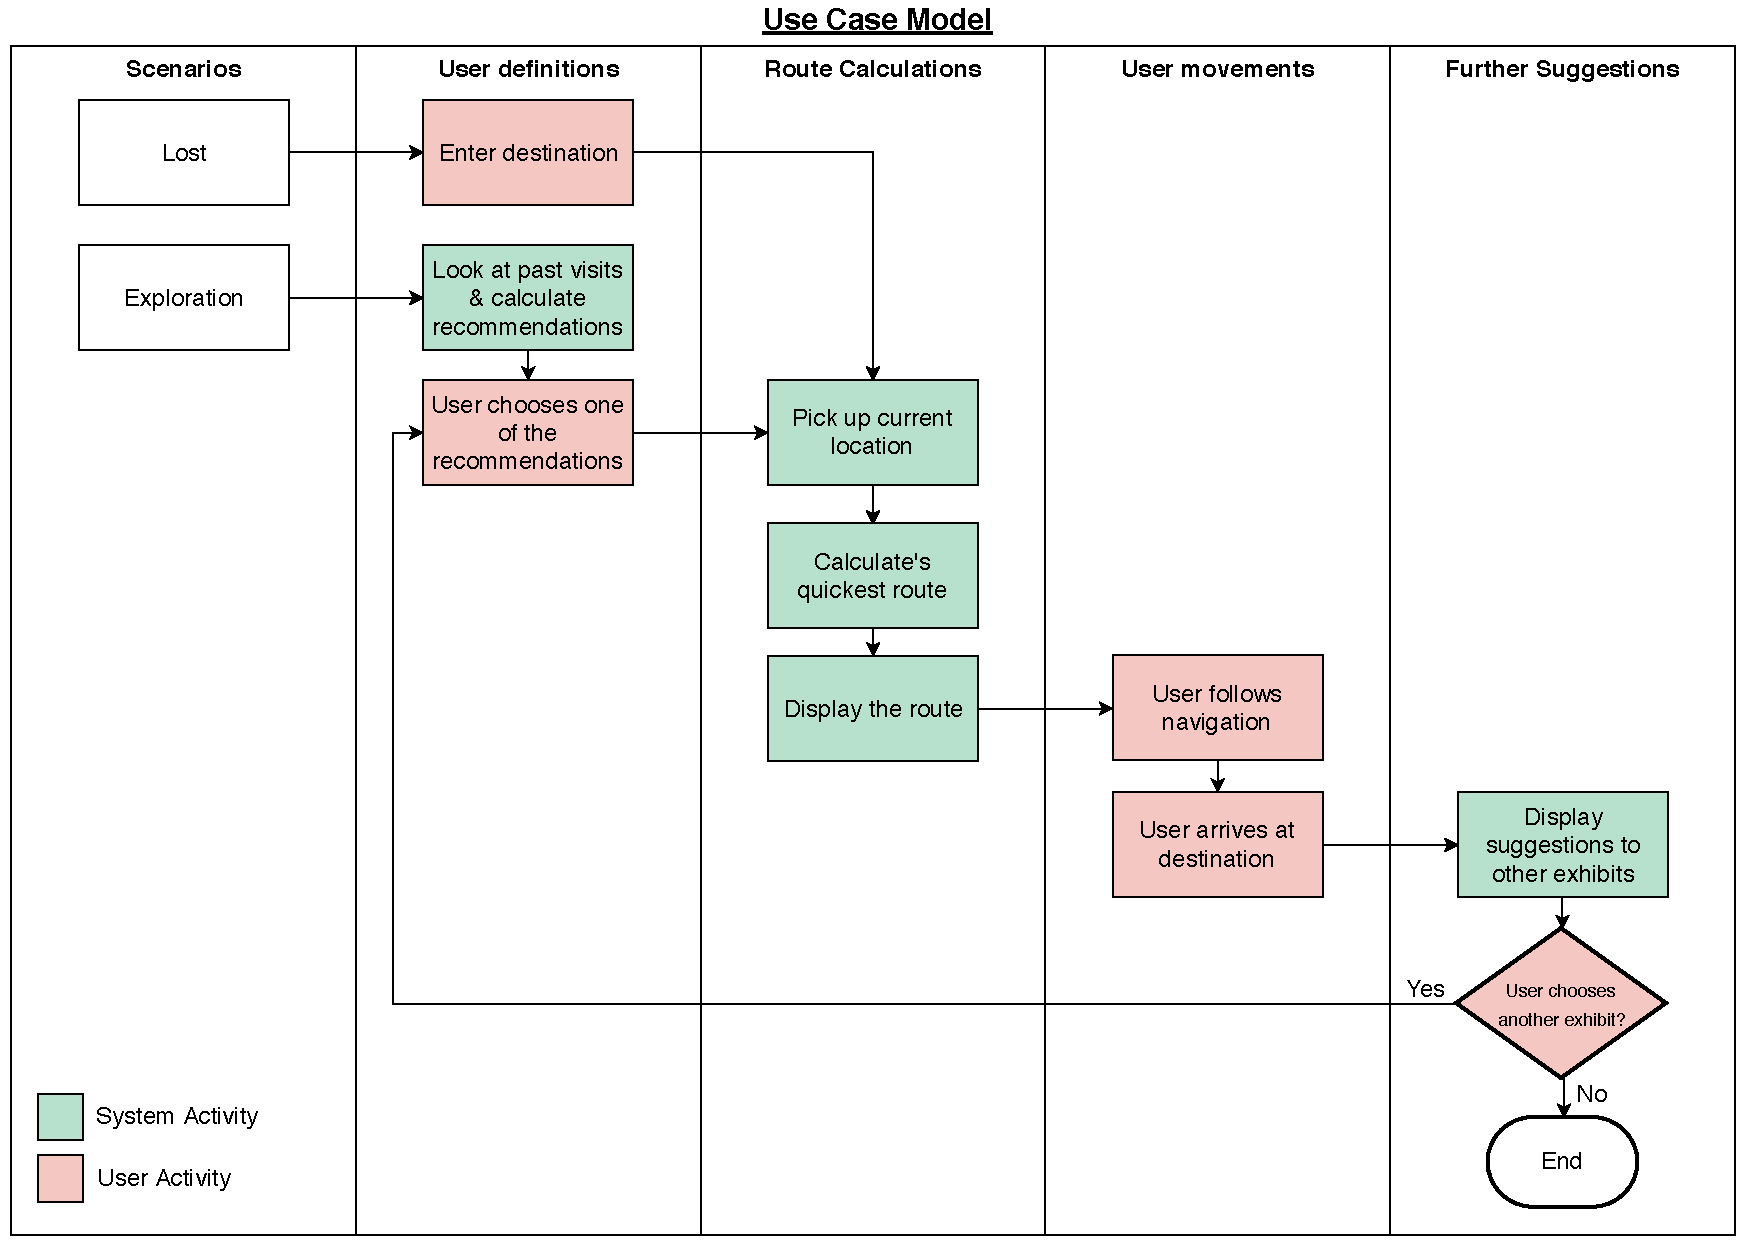
\includegraphics[width=60mm, height=100mm]{use_case.pdf}
		\begin{center}
		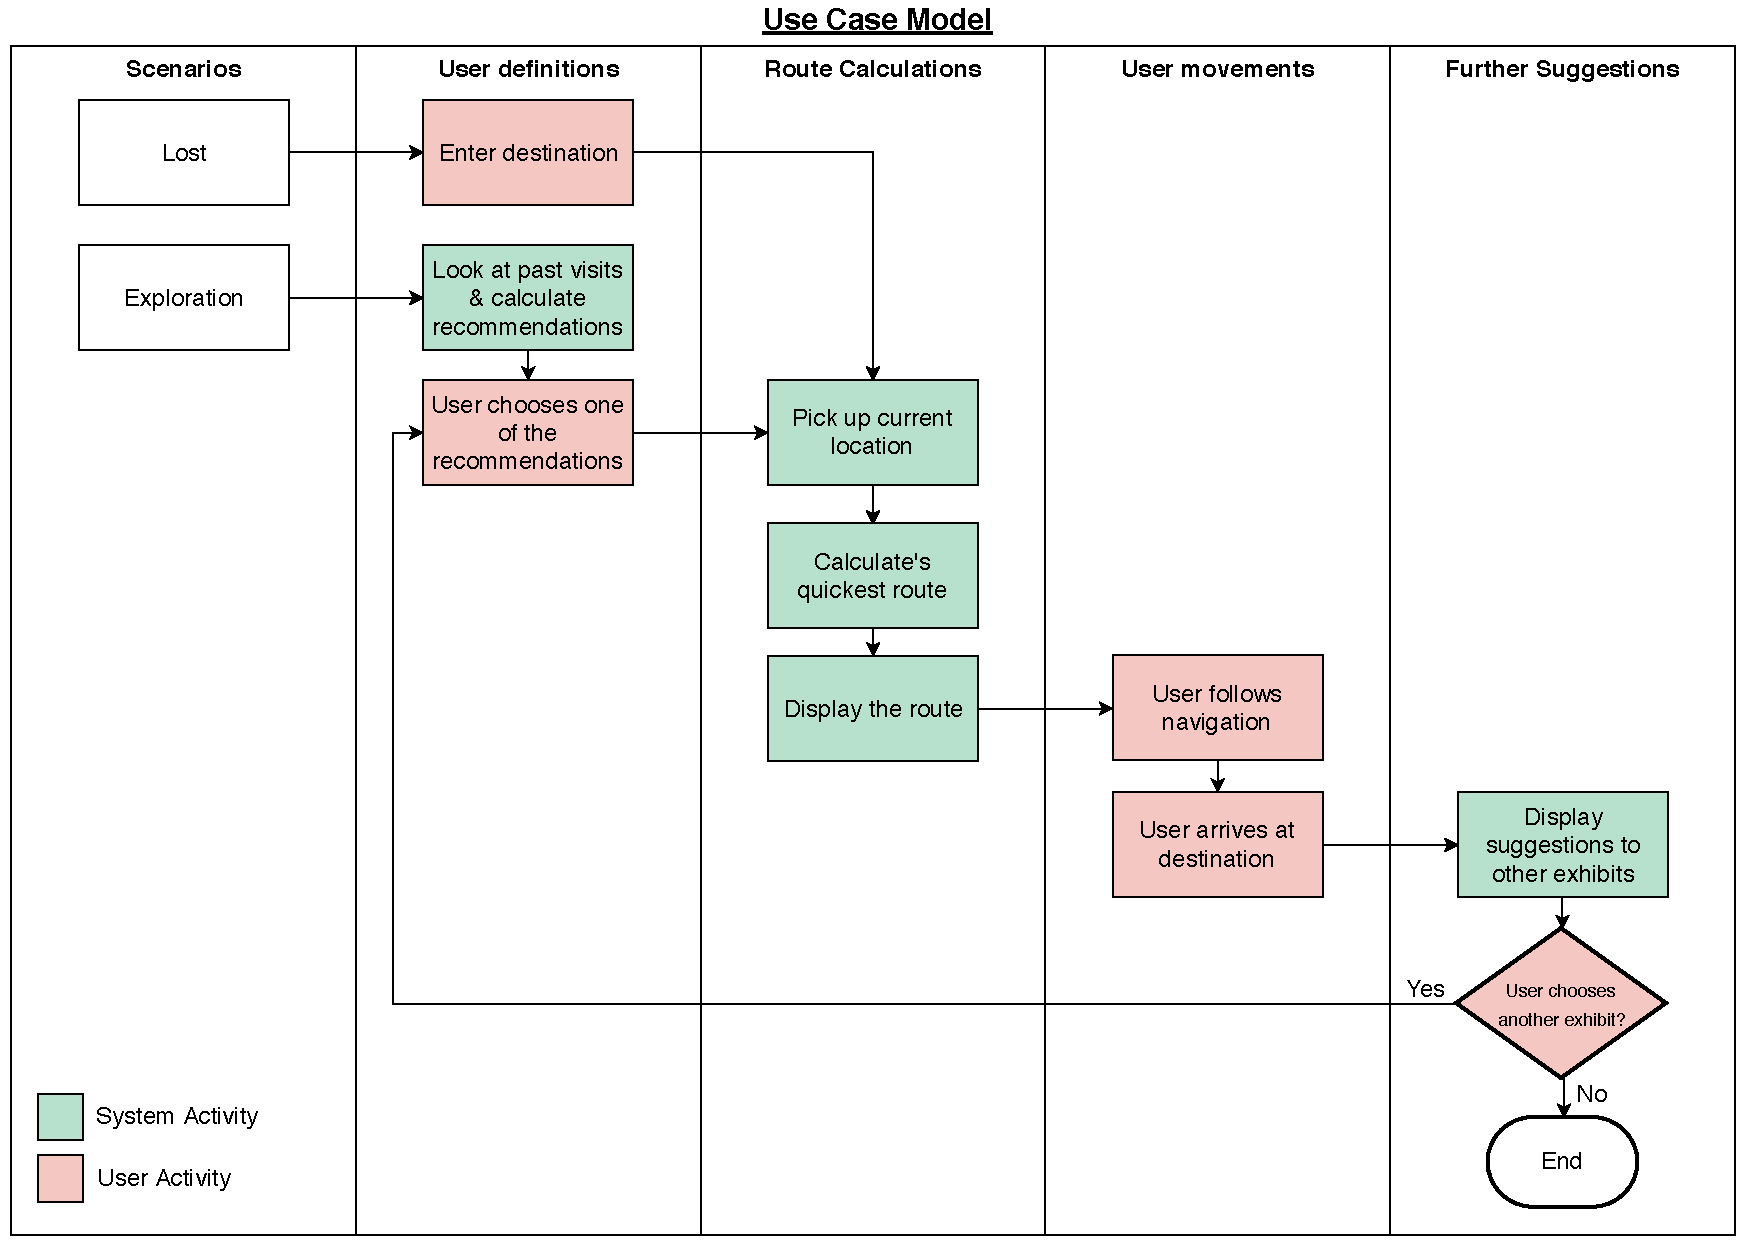
\includegraphics[width=110mm, height=80mm]{use_case.pdf}
		\end{center}
	\end{frame}

	\begin{frame}
		\framesubtitle{Model-View Controller}
		\begin{center}
		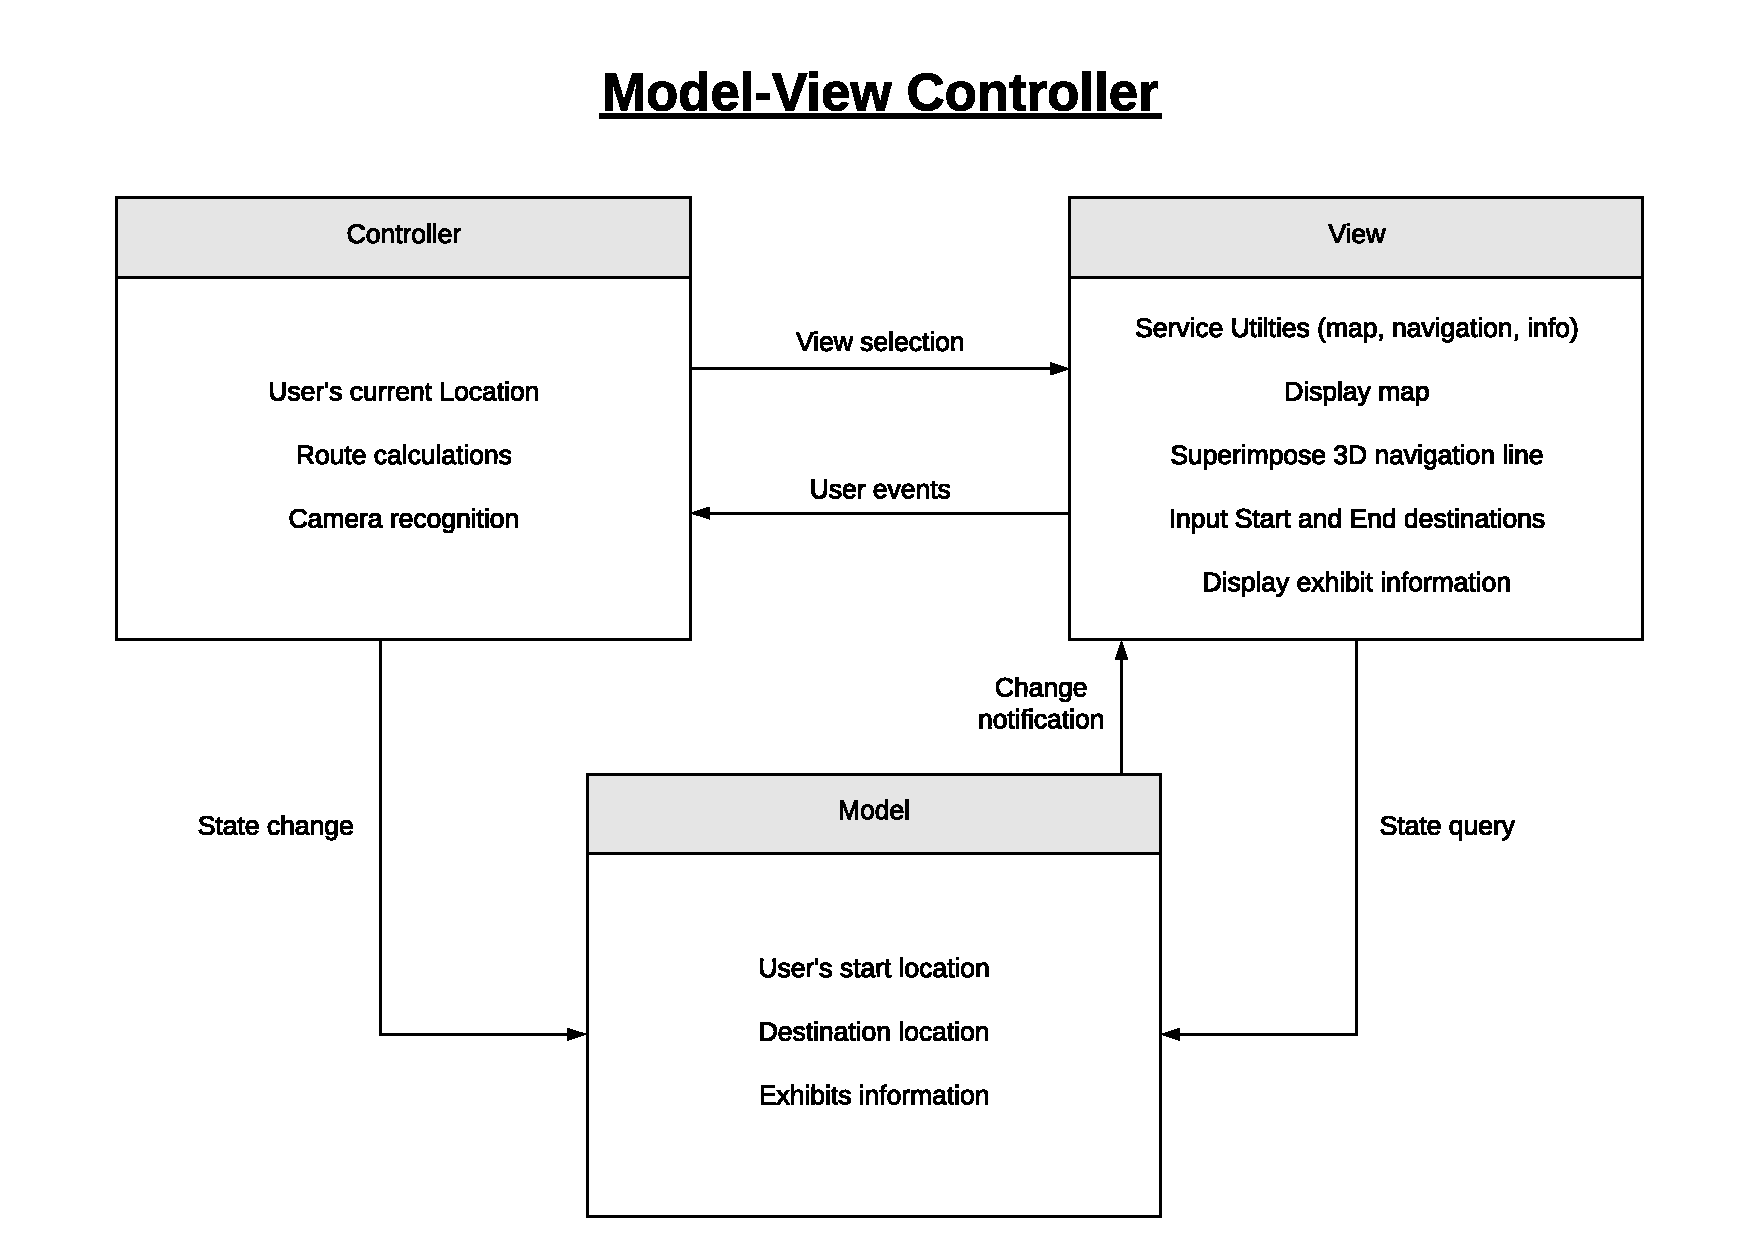
\includegraphics[width=110mm, height=80mm]{mvc.pdf}
		\end{center}
	\end{frame}

	\section{Development Process, Testing \& Outcomes}
	\subsection{Development Process}
	\begin{frame}
	    \frametitle{Development Process \& Testing}
		\begin{itemize}
			\item Used Agile/Scrum instead of Waterfall
			\item 4 Sprints Conducted
			\item TDD approach
			\begin{itemize}
				\item Unit
				\item Integration
				\item Regression
				\item Performance \& Stress
				\item User Acceptance (UAT)
			\end{itemize}
		\end{itemize}
	\end{frame}

	\subsection{Outcomes}
	\begin{frame}
		\frametitle{Outcomes}

		\framesubtitle{Sprints Conducted}
		\begin{itemize}
			\item Arduino hardware construction and Bluetooth
			\item Navigation using A* path-finding algorithm
			\item AR: Rendering objects on screen
		\end{itemize}
	\end{frame}

	\section{Evaluation}
	\subsection{Evaluation}
		\begin{frame}
			\frametitle{Evaluation}
			\begin{itemize}
				\item High technical standard in the back-end
				\item Very "agile" in moving things between sprints to accommodate changes
				\item Good feedback from industry professionals and users
				\item Executed plans as of our proposal according to stakeholders and user requirements
			\end{itemize}
		\end{frame}

	\subsection{Questions}
	\begin{frame}
		\begin{center}
			\Huge Questions?
		\end{center}
	\end{frame}
\end{document}
